\vspace{-10pt}
\chapter{Market Analysis}\label{chap:Market_analysis}
\vspace{-10pt}

% This should be performed first, as it lays the foundation for the motivation of all technical development

% \begin{itemize}
%     \item It identifies the market need for your mission
%     \item \textbf{Crucial}: market analysis always leads to more/new requirements!
%     \item You should identify all stakeholders - all those that are affected by and can affect the mission
%     \item $\rightarrow$ Extends beyond customers: users, regulatory agencies (constraints stakeholders), etc.
%     \item Prioritize the stakeholders into key and non-key
%     \item It is suggested to create an interest-influence graph/stakeholder map
%     \item Identify market segments and competitors $\rightarrow$ perform mission SWOT analysis to distinguish position in market
%     \item Given the user requirements, how competitive is your product to be?
%     \item With a (minor) change, can your product become more competitive or more valuable? $\rightarrow$ cost trade-off
% \end{itemize}



 
The economic viability of any new aerial system is determined by two interdependent factors: the size and structure of the market it addresses, and the cost at which the system can be produced and deployed to compete within that market. This chapter analyses the balloon interception market to establish the demand landscape and identify the technology gap. A product cost estimation in \autoref{sec:roi} then modifies those market-derived targets into concrete budget indications for the UAS design.  
 \vspace{-10pt}
\section{Problem Relevance and Operational Demand}
\label{subsec:demand}
 
Free-floating balloons create two distinct categories of airspace hazard that
motivate a dedicated interception capability.
 \vspace{-10pt}
\paragraph{Meteorological balloon drift:}
Approximately 900 radiosondes are launched globally every day by national weather services, each ascending until burst at 20-35 km and then descending \cite{WorldMeteorologicalOrganization2018GuideGuide}. Some of these drift into restricted airspace before reaching burst altitude, particularly near major airports situated within 20-50 km of launch sites. The resulting airspace closure protocol is equivalent in cost to any other airspace violation event: industry analyses place the direct cost of a single unplanned airport closure at \$100 per minute in airline operational losses alone, with total economy-wide
disruption costs from unplanned airport events estimated at \$30-34 billion annually in the US \cite{AirHelp2024CostEconomy, AirHelp20242023Overview}. 
 \vspace{-10pt}
\paragraph{Hybrid-use and smuggling balloons:}
Since 2023, large helium balloons repurposed for contraband delivery and hybrid airspace disruption have created a growing risk. The balloon incursions recorded in Lithuania forced the Vilnius International Airport to close for more than 60 hours and canceled over
350 flights affecting approximately 51000 passengers \cite{AlJazeera2025LithuaniaBelarus}. Revenue losses to Lithuanian aviation businesses were estimated at \texteuro{}2 million in 2025 \cite{BBCNews2025BalloonClosures}. Balloons entered Polish airspace on Christmas Eve 2025, forcing temporary airspace restrictions\cite{EuromaidanPress2025PolandEve}.
 
Both scenarios share a critical operational gap: no existing commercial system provides non-destructive, debris-free, UAS-based interception of large free-floating balloons in civilian airspace.
 
 \vspace{-10pt}
\subsection*{Existing Solutions and Technology Gap}
\label{subsec:solutions}
 
Table \ref{tab:market_solutions} surveys the principal categories of existing counter-balloon and counter-UAS technology and their applicability to the present mission.
 
\begin{longtable}{@{}p{3.2cm}p{3.4cm}p{2.5cm}p{5.5cm}@{}}
\caption{Comparison of existing airspace threat mitigation technologies
  against the requirements.}
\label{tab:market_solutions} \\

\toprule
\textbf{Technology} & \textbf{Representative system} & \textbf{Unit cost (approx.)} & \textbf{Gap vs.\ project requirements} \\
\midrule
\endfirsthead

\toprule
\textbf{Technology} & \textbf{Representative system} & \textbf{Unit cost (approx.)} & \textbf{Gap vs.\ project requirements} \\
\midrule
\endhead

Kinetic interceptor (missile) &
  Patriot / Iron Dome &
  \$40k-\$3M per shot \cite{UAVDefence2025NewMicrowaves} &
  Explosive; creates uncontrolled debris; prohibited in civilian airspace \\[4pt]
 
Directed energy (laser) &
  Iron Beam (Rafael) &
  \$0.10-\$10 per shot \cite{UAVDefence2025NewMicrowaves} &
  Destroys envelope; uncontrolled descent; not certified for civilian use \\[4pt]
 
Net-launching drone\newline(anti-drone) &
  Fortem DroneHunter F700,\newline ParaZero DefendAir, DroneCatcher &
  \$1k-\$3k per capture \cite{UAVDefence2025NewMicrowaves} &
  Designed for small rigid UAVs ($<$1 m); net geometry unsuitable for
  2-6 m elastic balloon envelopes; no buoyancy management post-capture \\[4pt]
 
Ground-based net gun &
  UAVOS capture net &
  \$5k-\$50k system &
  Ground range $<$30 m; cannot reach 1-10 km altitude targets \cite{AirsightSecurity2024AirTechnology} \\[4pt]
 
Manual helicopter\newline interception &
  Ad hoc, case by case &
  \$2k-\$10k per sortie &
  Pilot safety risk; high cost; 30-60 min response time; not scalable \\[4pt]


\bottomrule
\end{longtable}
\normalsize
 
Small UAV interception has already been demonstrated, but no system addresses the very different problem of a large, buoyant target floating uncontrolled. This constitutes a clear and documented technology gap.
 
 \vspace{-10pt}
\subsection*{Market Context and Customer Segments}
\label{subsec:market}
 
The extended counter-UAS market provides context for investment enthusiasm and technology readiness. Counter-drone system market valuations range from \$1.8 billion \cite{FutureDataStats2024Counter-Drone2024} to \$3.2 billion \cite{GrandViewResearch2025Anti-Drone20252033} in 2024-2025, with CAGR projections of 22-27\% through 2030-2033. UAV-based interception platforms are the fastest growing sub-segment, at a projected 26\% CAGR \cite{MordorIntelligence2025Anti-Drone20252030}, driven by the need for flexible, deployable, range-independent neutralization tools that ground-fixed systems cannot provide.
 
Three macro-level drivers are directly relevant to the balloon interception mission:
 
\begin{itemize}
  \item \textbf{Hybrid airspace disruptions:} Balloon campaigns have demonstrated that state-tolerated actors can disrupt civilian aviation repeatedly at low cost. Defence ministries have responded with sanctions and declarations, but no fielded solution exists yet \cite{CNN2025BalloonSays, AlJazeera2025LithuaniaBelarus}. Lithuania announced a \texteuro{}1 million prize for effective balloon interception concepts in December 2025 \cite{RFE/RLBelarusService2025UpBoth}.
 
  \item \textbf{Airport airspace protection:} Detection solutions currently account for 55\% of counter-UAS market revenue \cite{MordorIntelligence2025Anti-Drone20252030}, but airport operators increasingly demand paired neutralization capability, the gap that the present UAS is designed to fill for the balloon-specific threat.
 
  \item \textbf{Non-destructive civilian compliance:} Regulatory frameworks in Europe (EASA) and the US (FAA Part 107) prohibit explosive, kinetic, or jamming-based countermeasures in civilian airspace without special waivers. This disqualifies the dominant military solutions and creates a protected market niche.
\end{itemize}
 
 

Five customer segments have been identified whose operational requirements and budget constraints collectively define the system's design envelope. Despite facing different threat scenarios (from uncoordinated meteorological drift to deliberate state-directed incursions), all segments share a common core requirement summary satisfied by BELLONA.

 
\begin{longtable}{@{}p{5cm}p{5cm}p{5cm}@{}}
\caption{Primary customer segments and the balloon threat scenario relevant to each.}
\label{tab:customers} \\

\toprule
\textbf{Customer segment} & \textbf{Balloon threat} & \textbf{Deployment scenario} \\
\midrule
\endhead

National meteorological services &
  Own escaped radiosondes drifting toward controlled airspace &
  Reactive recovery; preserves equipment and data \\[4pt]

Airport operators (civilian) &
  Stray meteorological balloon or hybrid platform getting close to the runway approach cone &
  On-call standby; triggered by radar/ATC alert \\[4pt]

Border security agencies &
  State-directed hybrid balloon incursions carrying contraband or GPS probes &
  Proactive patrol along border corridors; coordinated with military radar \\[4pt]

Critical infrastructure operators &
  Accidental or deliberate balloon intrusions near power plants, data centers &
  Standby; triggered by perimeter sensor \\[4pt]

Scientific balloon operators &
  Escaped zero-pressure or latex balloon drifting beyond the planned flight zone &
  Planned recovery asset for high-value payloads \\

\bottomrule
\end{longtable}

\vspace{-15pt}
\section{Stakeholder Analysis}
\label{subsec:stakeholders}

Beyond direct customers, the system's development and deployment involve stakeholders whose influence or exposure to the project can affect its approval, market access, and operational viability. \autoref{tab:stakeholders} maps these groups by interest level and institutional power to shape project outcomes. The power-interest map in \autoref{fig:stakeholder_map} provides a visual prioritization of these stakeholders, distinguishing those requiring active engagement from those requiring monitoring only.

\begin{longtable}{@{}p{3.5cm}p{1.4cm}p{1.3cm}p{1.4cm}p{1.3cm}p{4.5cm}@{}}

\caption{Stakeholder power-interest matrix for the UAS balloon interception system, with explicit key/non-key prioritization. Interest: the degree to which the stakeholder is affected by or cares about the system. Power: ability to enable or block development and deployment.}
\label{tab:stakeholders} \\

\toprule
\textbf{Stakeholder} & \textbf{Type} &
  \textbf{Interest} & \textbf{Power} &
  \textbf{Priority} & \textbf{Key concern} \\
\midrule
\endfirsthead

\toprule
\textbf{Stakeholder} & \textbf{Type} &
  \textbf{Interest} & \textbf{Power} &
  \textbf{Priority} & \textbf{Key concern} \\
\midrule
\endhead

Airport operators & Customer & High & Medium & Key & Certified intercept; zero debris over runways \\[4pt]
 
National border\newline agencies & Customer & High & High & Key & Foreign incursions; minimal training burden \\[4pt]
 
EASA / national CAAs & Regulator & Medium & Very high & Key & Primary deployment gating authority \\[4pt]
 
defence ministries & Funder / Enabler & High & High & Key & Hybrid threat response; procurement and funding (Lithuania \texteuro{}1M prize \cite{RFE/RLBelarusService2025UpBoth}) \\[4pt]
 
Eurocontrol / ANSPs & Regulator / Enabler & Medium & High & Key & Airspace integration in controlled airspace \\[4pt]
 
National meteorological services & Customer & Medium & Low & Non-key & Radiosonde recovery; high cost-sensitivity \\[4pt]
 
Defence prime\newline contractors & Competitor / Partner & Medium & Medium & Non-key & May seek to acquire at scale \\[4pt]
 
Local communities & Affected party & Low & Low & Non-key & Noise and overflights; managed via 65dB limit \\[4pt]
 
Balloon smuggling\newline networks & Adversarial & High & Low & Non-key & Disrupted by system; altitude shift \\

\bottomrule
\end{longtable}

\begin{figure}[H]
\centering
\vspace{-10pt}
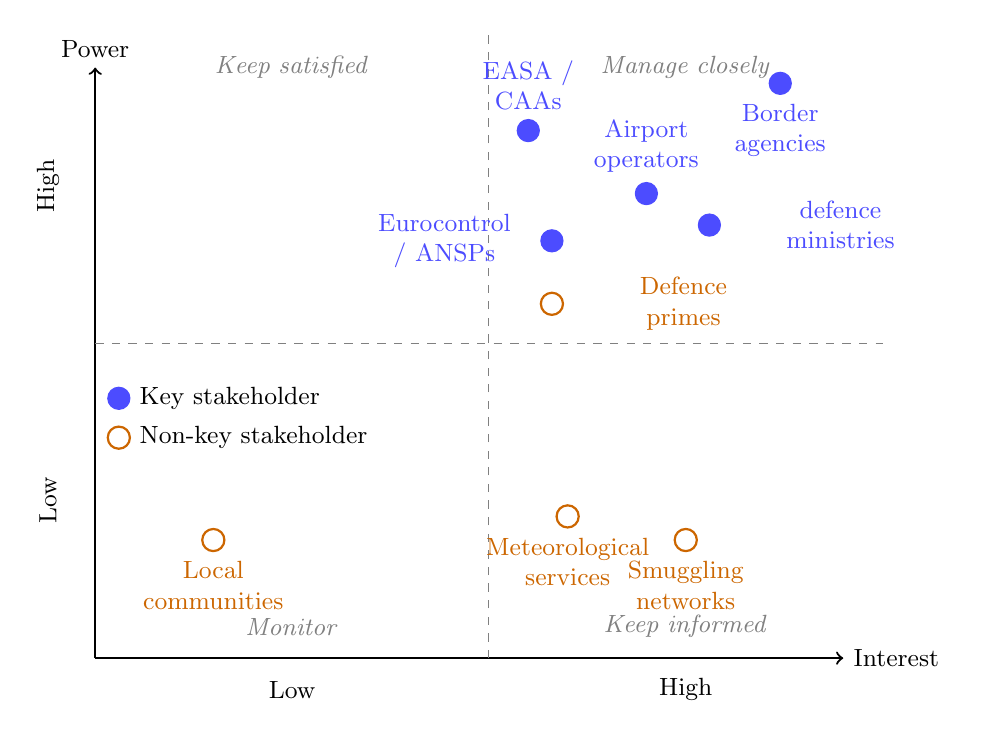
\begin{tikzpicture}[
    font=\small,
    node distance=0pt,
    every node/.style={align=center}
]
 
 
\draw[thick,->] (0,0) -- (9.5,0) node[right] {Interest};
\draw[thick,->] (0,0) -- (0,7.5)  node[above]  {Power};
 
 
\draw[dashed, gray] (5,0) -- (5,8);
\draw[dashed, gray] (0,4) -- (10,4);
 
 
\node[gray, text width=3.5cm] at (2.5,7.5) {\textit{Keep satisfied}};
\node[gray, text width=3.5cm] at (7.5,7.5) {\textit{Manage closely}};
\node[gray, text width=3.5cm] at (2.5,0.4) {\textit{Monitor}};
\node[gray, text width=3.5cm] at (7.5,0.4) {\textit{Keep informed}};
 
 
\filldraw[blue!70] (7.0,5.9) circle (4pt)
    node[above=4pt, text width=2.8cm] {Airport\\operators};
 
\filldraw[blue!70] (8.7,7.3) circle (4pt)
    node[below=4pt, text width=2.8cm] {Border\\agencies};
 
\filldraw[blue!70] (5.5,6.7) circle (4pt)
    node[above=4pt, text width=2.5cm] {EASA /\\CAAs};
 
\filldraw[blue!70] (7.8,5.5) circle (4pt)
    node[right=4pt, text width=2.8cm] {defence\\ministries};
 
\filldraw[blue!70] (5.8,5.3) circle (4pt)
    node[left=4pt, text width=2.2cm] {Eurocontrol\\/ ANSPs};
 
 
\draw[orange!80!black, thick] (6.0,1.8) circle (4pt)
    node[below=4pt, text width=2.5cm] {Meteorological\\services};
 
\draw[orange!80!black, thick] (5.8,4.5) circle (4pt)
    node[right=4pt, text width=2.8cm] {Defence\\primes};
 
\draw[orange!80!black, thick] (1.5,1.5) circle (4pt)
    node[below=4pt, text width=2.2cm] {Local\\communities};
 
\draw[orange!80!black, thick] (7.5,1.5) circle (4pt)
    node[below=4pt, text width=2.8cm] {Smuggling\\networks};
 
 
\node at (2.5,-0.4) {Low};
\node at (7.5,-0.4) {High};
\node[rotate=90] at (-0.6,2.0) {Low};
\node[rotate=90] at (-0.6,6.0) {High};
 
 
\filldraw[blue!70] (0.3,3.3) circle (4pt);
\node[right=4pt] at (0.3,3.3) {Key stakeholder};
\draw[orange!80!black, thick] (0.3,2.8) circle (4pt);
\node[right=4pt] at (0.3,2.8) {Non-key stakeholder};
 
\end{tikzpicture}
\vspace{-10pt}
\caption{Power-interest map of project stakeholders. Key ones require active engagement; non-key ones require periodic communication only.}
\vspace{-10pt}
\label{fig:stakeholder_map}
\end{figure}
\section{SWOT Analysis}
\label{subsec:swot}

The SWOT analysis below evaluates the proposed UAS balloon interception system from a market and product perspective. Its purpose is to consolidate the findings of the previous subsections into a structured framework.
\begin{table}[H]
\centering
\caption{SWOT analysis of the proposed UAS balloon interception system: strengths and weaknesses.}
\vspace{-10pt}
\label{tab:swot_strengths_weaknesses}
\begin{tabular}{@{}p{7.6cm}|p{7.6cm}@{}}
\toprule
\textbf{Strengths} & \textbf{Weaknesses} \\
\midrule
\vspace{-0.7\baselineskip}
\begin{itemize}[leftmargin=*,nosep,topsep=0pt,partopsep=0pt]
  \item Only known concept combining civilian airspace compliance,
        non-destructive interception, and a sub-\texteuro{}5000 system
        Cost: no direct commercial competitor exists.
  \item Applicable to both meteorological and hybrid/smuggling balloon
        risks; a single platform addresses multiple customer segments
        (airports, border agencies, met services).
  \item Electric propulsion and reusable consumables align with tightening European sustainability and noise regulations, lowering regulatory risk during certification.
  \item Low per-sortie cost (\texteuro{}$<$500 target) is an order of magnitude below helicopter alternatives (\$2k-\$10k), making routine deployment economically rational for operators.
\end{itemize}
&
\vspace{-0.7\baselineskip}
\begin{itemize}[leftmargin=*,nosep,topsep=0pt,partopsep=0pt]
  \item Balloon-specific interception at 1-20 km altitude imposes severe endurance and payload requirements on the pricing; a low cost threshold may be unachievable for the full altitude range without compromising capability.
  \item No flight-heritage for this exact mission profile; the technology readiness level (TRL) is low, increasing development risk and timeline uncertainty.
  \item Buoyancy or payload management post-capture adds structural and energy demands not present in anti-drone analogues, complicating gripper and power budget design.
  \item Prototype is a single unit; it lacks the redundancy and swarm capability needed to counter coordinated multi-balloon incursions (up to 25 balloons in a single night \cite{RFE/RLBelarusService2025UpBoth}).
\end{itemize}
\\
\bottomrule
\end{tabular}
\end{table}
 \begin{table}[H]
\centering
\caption{SWOT analysis of the proposed UAS balloon interception system: opportunities and threats.}
\vspace{-10pt}
\label{tab:swot_opportunities_threats}
\begin{tabular}{@{}p{7.6cm}|p{7.6cm}@{}}
\toprule
\textbf{Opportunities} & \textbf{Threats} \\
\midrule
\vspace{-0.7\baselineskip}
\begin{itemize}[leftmargin=*,nosep,topsep=0pt,partopsep=0pt]
  \item Lithuania's \texteuro{}1 million public prize for effective balloon interception solutions \cite{RFE/RLBelarusService2025UpBoth} provides a concrete market entry point.
  \item The counter-UAS market is growing at 22-27\% CAGR \cite{MordorIntelligence2025Anti-Drone20252030, GrandViewResearch2025Anti-Drone20252033}; UAV-based platforms are the fastest-growing segment at 26\% CAGR, indicating strong investor and procurement appetite.
  \item Regulatory gaps responses to hybrid balloon threats create first-mover advantage for a fielded, certified civilian solution.
  \item Capability upgrades for premium customer segments without full redesign.
\end{itemize}
&
\vspace{-0.7\baselineskip}
\begin{itemize}[leftmargin=*,nosep,topsep=0pt,partopsep=0pt]
  \item If hybrid balloon campaigns are resolved diplomatically or by existing military assets, near-term demand for a civilian UAS solution may stall before market entry.
  \item Established defence primes (Fortem, ParaZero, Elbit) could pivot their existing net-capture drone platforms to the balloon intercept mission, bringing significant investment and brand recognition.
  \item EASA BVLOS certification for autonomous interception is a long regulatory process; delays could make the prototype commercially non-viable before certification is obtained.
\end{itemize}
\\
\bottomrule
\end{tabular}
\end{table}
The SWOT analysis leads to additional requirements that complement the top-level specification and can be found in \autoref{tab:stakeholder-requirements}.


 \vspace{-10pt}
\section{Competitive Positioning Summary}
\label{subsec:positioning}
 
The project occupies a unique position at the intersection of three underserved requirements: (i) civilian airspace legal compliance,
(ii) non-destructive balloon-specific interception, and (iii) low cost. No commercial product currently satisfies all three simultaneously. The closest analogues, net-launching anti-drone interceptors, are designed for targets about 100$\times$ smaller in cross-section and provide no buoyancy management. The total addressable market is represented by the combination of the rapidly growing counter-UAS sector and the presence of hybrid balloon threats, for which states are actively seeking technical solutions and have committed public funding to speed up their development.



% \subsection{Market-Derived Design Implications}
% \label{sec:market_design_implications}

% The market analysis is not only used to justify the relevance of BELLONA, but also to derive design implications for the system. The identified customer segments impose different operational priorities, such as low acquisition cost for meteorological services, fast response for airport operators, repeated deployment capability for border agencies, and low disturbance for communities near sensitive infrastructure. These market needs are therefore translated into requirements and trade-off drivers in \autoref{tab:market_design_implications}.

% \begin{table}[H]
% \centering
% \caption{Market-derived design implications for the BELLONA system.}
% \label{tab:market_design_implications}
% \begin{tabular}{p{0.25\textwidth} p{0.32\textwidth} p{0.33\textwidth}}
% \toprule
% \textbf{Market finding} & \textbf{Design implication} & \textbf{Requirement or trade-off impact} \\
% \midrule
% Airport operators require rapid response to minimise airspace disruption. 
% & The system shall be deployable on-site and able to intercept shortly after target acquisition. 
% & Drives intercept time, mission readiness, launch procedure, and operator workload. \\

% Border agencies may face repeated or coordinated balloon incursions. 
% & The system shall be reusable, resettable, and suitable for repeated missions without major repair. 
% & Drives reusability, modularity, maintenance effort, and per-sortie cost. \\

% Meteorological services and smaller operators are cost-sensitive. 
% & The system shall remain affordable in acquisition and operation. 
% & Drives the \euro 5000 flying-component cost target and \euro 500 per-use cost target. \\

% Civilian airspace operation requires regulatory acceptability. 
% & The system shall avoid destructive, explosive, or high-collateral-damage interaction methods. 
% & Drives non-pyrotechnic interaction, controlled descent, debris prevention, and manual override. \\

% Local communities and infrastructure operators are affected by overflight, noise, and falling debris. 
% & The system shall minimise disturbance and avoid creating secondary hazards. 
% & Drives low-noise operation, controlled recovery, debris prevention, and safe recovery-zone selection. \\

% No existing commercial solution addresses large balloon interception and recovery. 
% & The concept should prioritise balloon-specific interaction and post-contact control rather than generic counter-UAS capture. 
% & Drives interaction-mechanism selection, balloon material compatibility testing, and post-contact risk assessment. \\
% \bottomrule
% \end{tabular}
% \end{table}

% The resulting design implication is that BELLONA should not be optimised for interception alone. A commercially relevant solution must combine fast deployment, low cost, controlled recovery, reusability, and regulatory compatibility. These market-derived drivers are carried forward into the requirements in \autoref{ch:Requirements} and into the Midterm trade-off criteria.